%\setcounter{chapter}{13} % "N" (14th letter, but latex first increments -> 14-1=13)
\chapter{Design Description \& Frame Construction } \label{ch:design}

The implemented architecture establishes a complete \textsf{OFDM} transceiver operating in baseband \autocite{Cimini1985}. To mimic a realistic transmission environment, the system simulates passband transmission through digital upconversion and downconversion steps. The system is logically divided into two primary processing blocks: the transmission chain and the reception chain.

\section{Transmission Chain}%
\label{sec:Transmission Chain}
\fileTeXtured{custom\_function/transmit/transmitter.m}

The transmission process is encapsulated within the \custommacro{transmitter} function. It orchestrates the transformation of raw binary data into a continuous time-domain waveform ready for the channel.

\begin{figure}[h]
    \fcapside[\FBwidth]{%
        \captionsetup{parskip = .5\baselineskip plus 1pt}%
        \caption[Time and Frequency Domain Representation of TX Symbols]{%
            Transmission Chain block diagram
        }%
        \label{fig:4}%
    }{%
        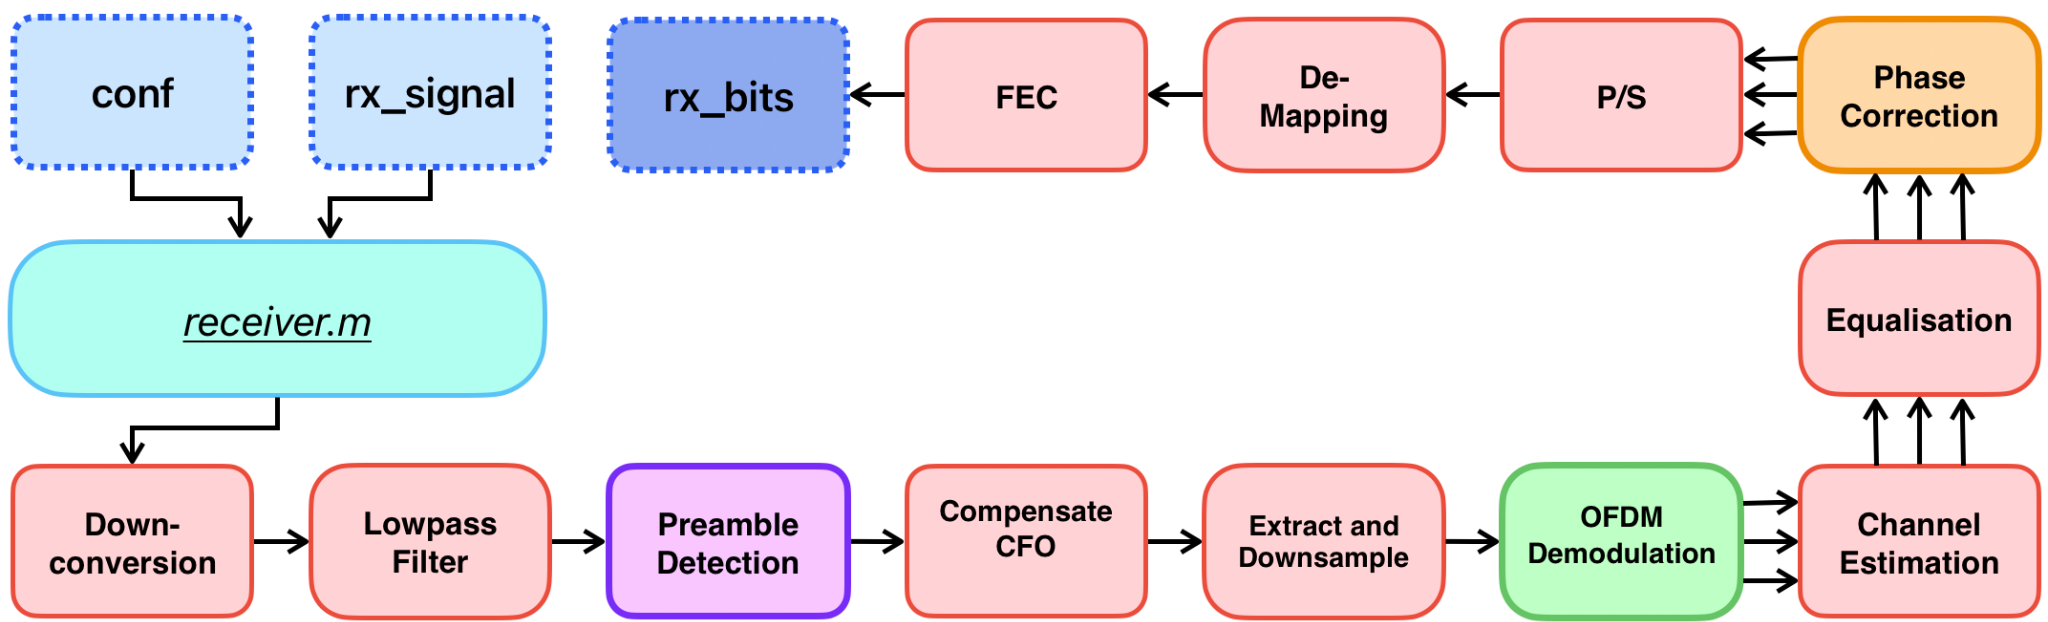
\includegraphics[width=0.80\textwidth]{figures/chap1_design/4.png}
    }
\end{figure}

\subsection{Payload Management and Concatenated FEC}%
\label{sub:Payload FEC}

The process begins with the generation or reception of the payload bits. All system parameters are centralized in \path{configurations.m}.
\begin{itemize}
    \item \textbf{Concatenated Coding:} If the Forward Error Correction (\textsf{FEC}) is enabled (via \path{conf.coding.use_fec}), the system employs a robust concatenated coding scheme implemented in \custommacro{channel\_encoder}. This architecture, along with its impact on overall link reliability, is analyzed in detail in \Cref{ch:performance}.
    
    \item \textbf{Symbol Mapping:} The encoded bit stream is mapped to complex symbols belonging to a configurable constellation (e.g., \textsf{QPSK}, \textsf{16-QAM}) defined in \path{conf.modulation}.
\end{itemize}

\begin{figure}[h]
    \fcapside[\FBwidth]{%
        \captionsetup{parskip = .5\baselineskip plus 1pt}%
        \caption[Time and Frequency Domain Representation of TX Symbols]{%
            OFDM Frame construction.
        }%
        \label{fig:4}%
    }{%
        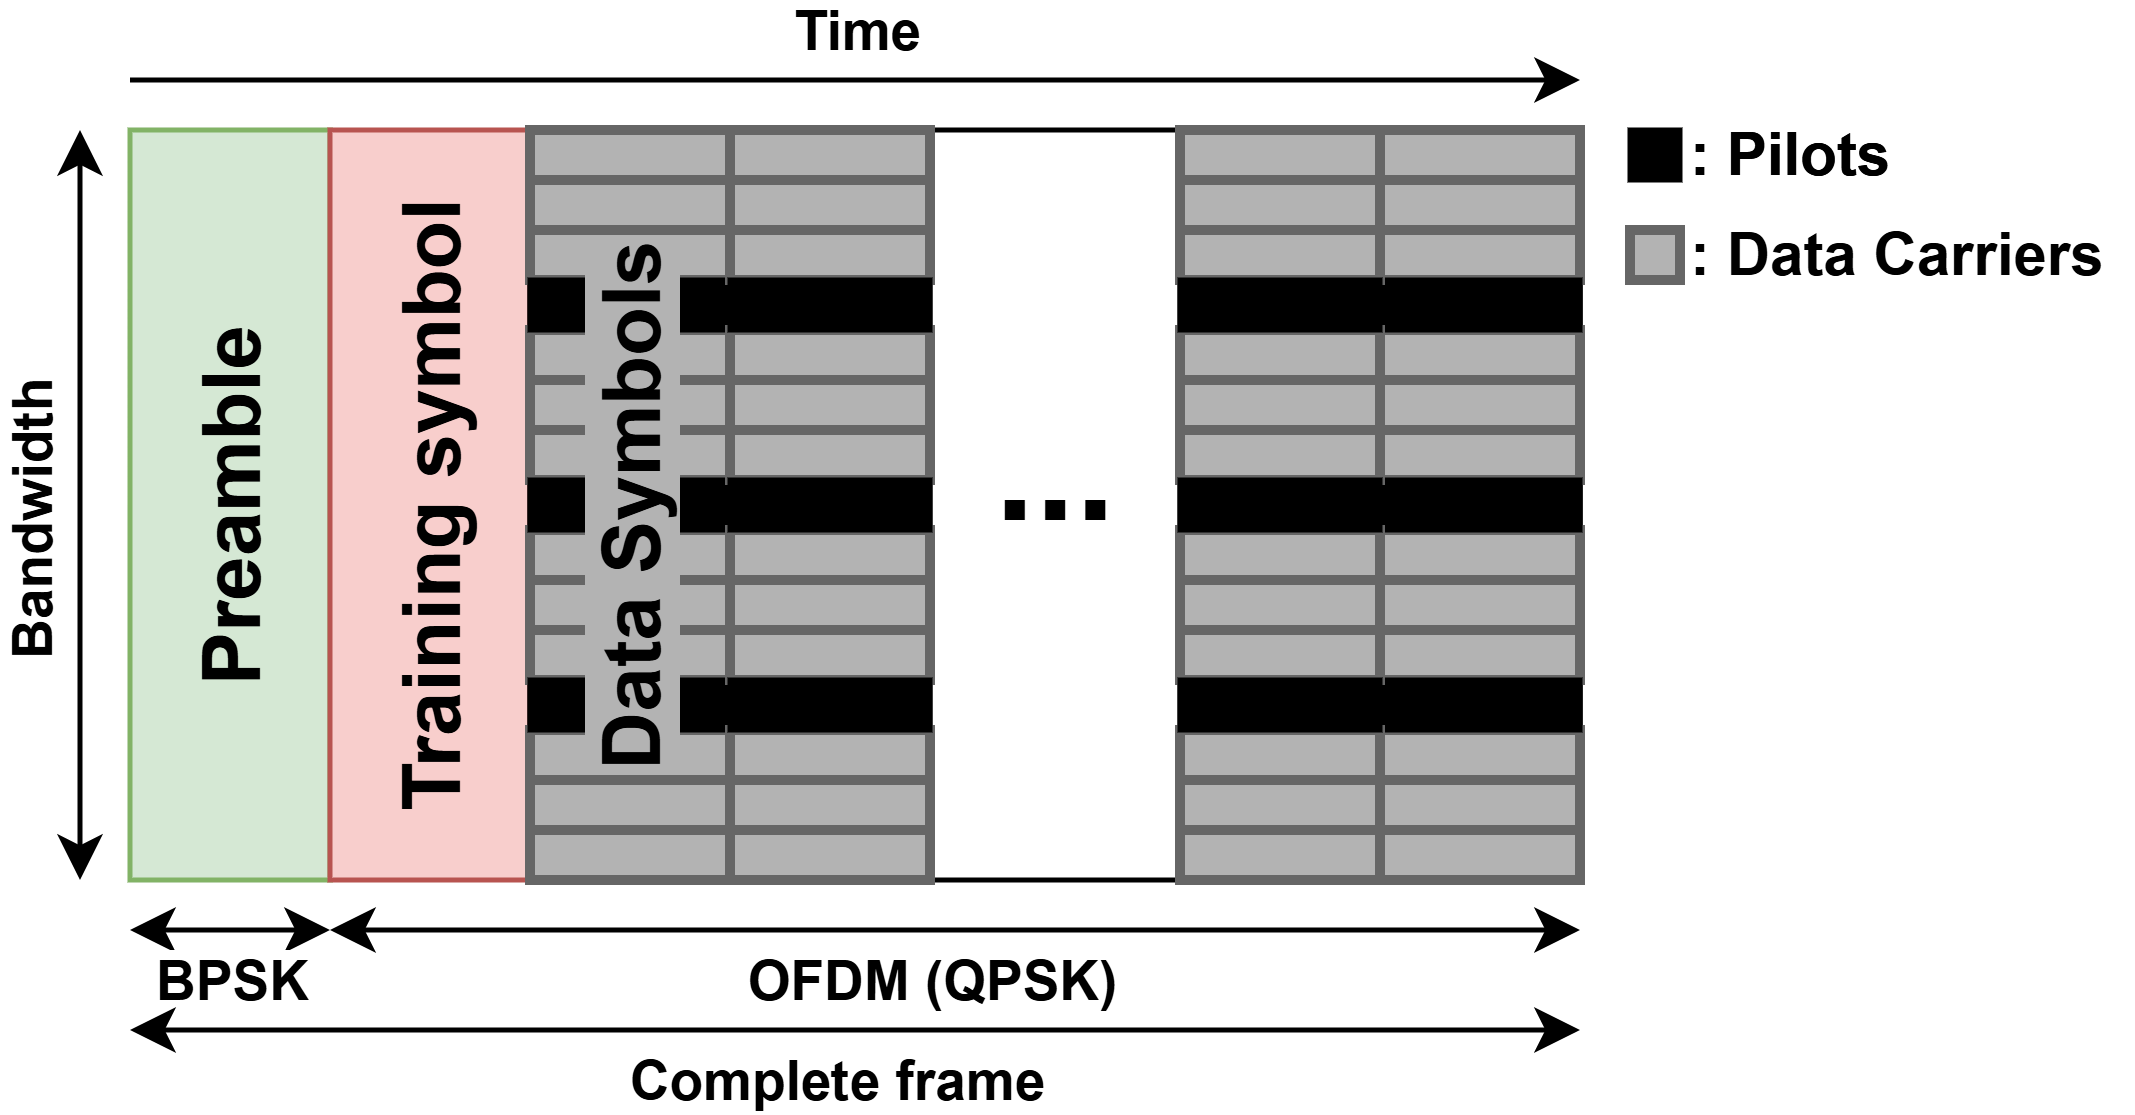
\includegraphics[width=0.70\textwidth]{figures/DrawIoSchematics/FrameStructure.png}
    }
\end{figure}

\subsection{OFDM Frame Construction}%
\label{sub:OFDM Frame Construction}
\fileTeXtured{.../ofdm\_tx\_frame\_with\_pilots.m}

The core signal construction is handled by the \custommacro{ofdm\_tx\_frame\_with\_pilots} function. This stage transforms the serial symbol stream into parallel frequency subcarriers:
\begin{enumerate}
    \item \textbf{Frequency Organization:} Data symbols are mapped onto the active subcarriers defined by the \path{conf.ofdm.psdMask}.
    \item \textbf{Training Symbol Insertion:} A dedicated \textbf{Training Symbol} (known to the receiver) is inserted as the very first OFDM symbol of the frame. This is strictly used for Channel Frequency Response (CFR) estimation and is distinct from the synchronization preamble.
    \item \textbf{Pilot Insertion:} Known pilot symbols are inserted at specific indices (defined in \path{conf.ofdm.pilotIndices}) within the data symbols. These pilots are crucial for tracking phase rotation caused by residual frequency offsets at the receiver.
    \item \textbf{IFFT \& Cyclic Prefix:} The frequency domain blocks are transformed into the time domain using the Inverse Fast Fourier Transform (\macro{ifft}). A Cyclic Prefix (CP) is appended to the beginning of each symbol to mitigate \emph{Inter-Symbol Interference} (ISI).
\end{enumerate}

\subsection{Finalization and Upconversion}%
\label{sub:Upconversion}

Following the OFDM modulation, the signal undergoes several conditioning steps in \custommacro{transmitter}:
\begin{enumerate}
    \item \textbf{Upsampling:} The OFDM signal is upsampled from the baseband bandwidth \autocite{Proakis2007} to the system sampling rate $f_s$ using \custommacro{ofdm\_tx\_resampling}.
    \item \textbf{Preamble Prepending:} To aid synchronization, a separate \textbf{Preamble sequence} (generated via LFSR) is prepended to the frame. Unlike the OFDM data, this preamble is a single-carrier sequence, upsampled and filtered with a Root-Raised Cosine (\textsf{RRC}) pulse to ensure good correlation properties.
    \item \textbf{Upconversion:} Finally, the signal is digitally upconverted to the carrier frequency $f_c$ by multiplying with a complex exponential $e^{j 2 \pi f_c t}$.
\end{enumerate}


\section{Reception Chain}%
\label{sec:Reception Chain}
\fileTeXtured{custom\_function/receive/receiver.m}

The receiver performs the inverse operations to recover the information from the noisy, distorted signal received from the channel.

\begin{figure}[h]
    \fcapside[\FBwidth]{%
        \captionsetup{parskip = .5\baselineskip plus 1pt}%
        \caption[Time and Frequency Domain Representation of TX Symbols]{%
            Reception chain block diagram.
        }%
        \label{fig:1}%
    }{%
        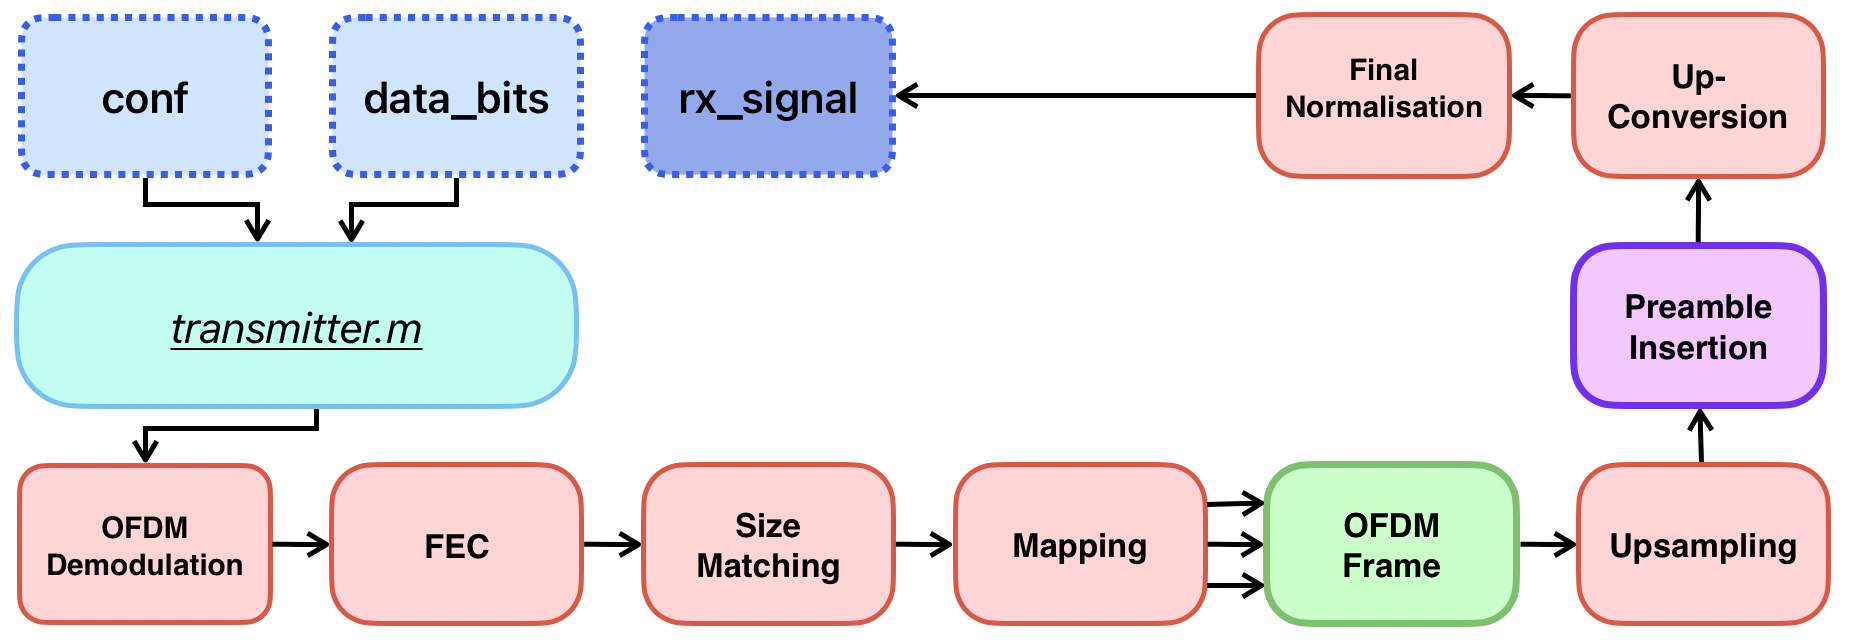
\includegraphics[width=0.80\textwidth]{figures/chap1_design/5.png}
    }
\end{figure}

\subsection{Downconversion and Filtering}%
\label{sub:Downconversion}

The received signal is first digitally downconverted from $f_c$ back to baseband. Immediately following the mixing, a low-pass filter is applied via \custommacro{ofdmlowpass} to remove double-frequency terms and out-of-band noise.

\subsection{Synchronization}%
\label{sub:Synchronization}
\fileTeXtured{custom\_function/receive/estimateTauAndCFO.m}

Before demodulation can occur, the receiver must synchronize in both time and frequency. This will be discussed in \Cref{ch:sync}.

\subsection{Channel Estimation and LMMSE Refinement}%
\label{sub:ChannelEst}
\fileTeXtured{.../receive/ChannelMetrics.m}

Once synchronized, the signal is resampled and the Cyclic Prefix is removed. The system then performs advanced channel estimation:
\begin{enumerate}
    \item \textbf{LS Estimation:} A Least Squares (LS) estimate is computed in \custommacro{channel\_estLS} by dividing the received \textbf{Training Symbol} (the first symbol of the frame) by the transmitted reference.
    \item \textbf{Asymmetric LMMSE Smoothing:} The LS estimate is refined using a practical \textsf{LMMSE} approach in \custommacro{ChannelMetrics}. This function:
    \begin{itemize}
        \item Transforms the LS estimate to the time domain (CIR).
        \item Centers the energy peak using circular shifts.
        \item Applies an \textbf{asymmetric window} defined by \path{conf.ch.back} (pre-cursors) and \path{conf.ch.length} (post-cursors) to filter out noise while preserving the multipath taps.
        \item Transforms back to the frequency domain to obtain the cleaned $\hat{H}_{\text{LMMSE}}$.
    \end{itemize}
\end{enumerate}
The data symbols are then equalized using the cleaned coefficients. Finally, residual phase rotations are tracked and corrected symbol-by-symbol using the pilot subcarriers via \custommacro{correctOFDMSymbolRotation}.

\begin{figure}[h]
    \fcapside[\FBwidth]{%
        \captionsetup{parskip = .5\baselineskip plus 1pt}%
        \caption[Time and Frequency Domain Representation of TX Symbols]{%
            Example of low resolution transmitted image.
        }%
        \label{fig:1}%
    }{%
        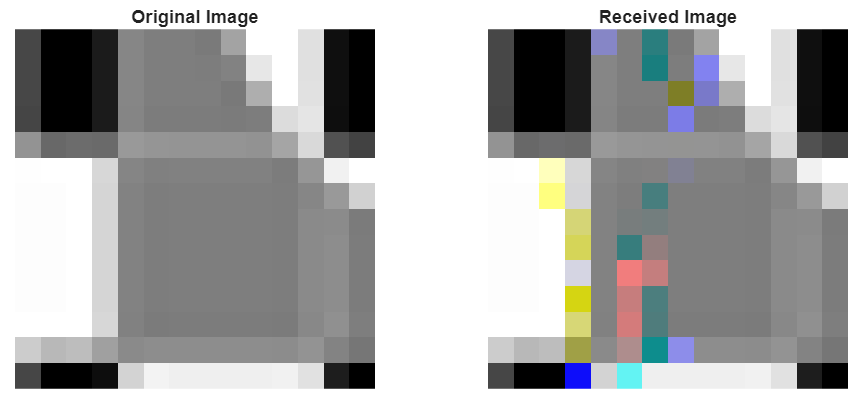
\includegraphics[width=0.80\textwidth]{figures/chap1_design/3.png}
    }
\end{figure}

\subsection{Decoding}%
\label{sub:Decoding}
\fileTeXtured{custom\_function/receive/channel\_decoder.m}

The equalized complex symbols are demapped into bits. If \textsf{FEC} is enabled, the bits are processed by the concatenated decoder (see \Cref{ch:coding}):
\begin{enumerate}
    \item \textbf{Viterbi Decoder:} The inner decoding step uses the Viterbi algorithm (hard decision) with a traceback depth defined in \path{conf.coding.traceBackDepth} to correct errors from the channel.
    \item \textbf{Reed-Solomon Decoder:} The outer decoding step processes the Viterbi output to correct any remaining block errors, providing the final estimated payload.
\end{enumerate}


\newpage
\section{Code Organization} \label{organization}
\begin{figure}[!ht]
    \fcapside[\FBwidth]{%
        \captionsetup{parskip = .5\baselineskip plus 1pt}%
        \caption[Project File Structure and Usage]{%
            \textbf{Structure and Usage Guide.}
            
            The project code is organized into a root directory containing the execution scripts and configuration, with modular functions separated by purpose.
            
            \textbf{Execution Flow:} The main entry point is \path{main.m}, which runs the complete image transmission experiment. It loads the image from \path{img/}, encodes it, transmits it (via audio or emulator), and reconstructs the received result. For performance analysis, \path{dbg_channelPlot.m} generates BER curves vs SNR, while \path{dbg_equalizationComp.m} compares different equalizer settings.

            \path{main_singleChannel al.m} tests OFDM transmission performance on a single channel by sending random payloads through the emulated channel at a fixed SNR. It computes Bit Error Rate (BER), Packet Error Rate (PER), and goodput over multiple packets.
            
            \textbf{Configuration:} All system parameters are centralized in \path{configurations.m}. This includes the OFDM setup (512 subcarriers, CP length), signal parameters ($f_s=48$kHz), and channel model selection. Modify this file to change the experiment conditions.
            
            \textbf{Core Modules:} The \path{custom_function/} directory houses the user-implemented logic. It is split into \path{transmit/} (encoder, frame builder) and \path{receive/} (synchronization, channel estimation, decoding). Helper scripts like \path{preamble_generate.m} reside in the root of this folder. The \path{provided_function/} directory contains the pre-compiled channel emulator and standard filters provided for the course.
        }%
        \label{fig:project-structure}%
    }{%
        \begin{tikzpicture}[dirtree]
            \node[directory] {OFDM Project/}
            child { node {configurations.m}}
            child { node {main.m}}
            child { node {main\_singleChannel.m}}
            child { node {dbg\_channelPlot.m}}
            child { node {dbg\_equalizationComp.m}}
            child { node[directory] {custom\_function/}
                child { node {preamble\_generate.m}}
                child { node {tfplotReImPhase.m}}
                child { node[directory] {receive/}
                    child { node {receiver.m}}
                    child { node {estimateTauAndCFO.m}}
                    child { node {ChannelMetrics.m}}
                    child { node {channel\_estLS.m}}
                    child { node {channel\_decoder.m}}
                    child { node {correctOFDMSymbolRotation.m}}
                    child { node {ofdm\_rx\_frame.m}}
                }
                child [missing] {} child [missing] {} child [missing] {} child [missing] {} child [missing] {} child [missing] {} child [missing] {} 
                child { node[directory] {transmit/}
                    child { node {transmitter.m}}
                    child { node {ofdm\_tx\_frame\_with\_pilots.m}}
                    child { node {channel\_encoder.m}}
                }
            }
            child [missing] {} child [missing] {} child [missing] {} child [missing] {} child [missing] {} child [missing] {} child [missing] {} child [missing] {} child [missing] {} child [missing] {} child [missing] {} child [missing] {}
            child [missing] {} child [missing] {}
            child { node[directory] {img/}
                child { node {test-image.bmp}}
                child { node {received\_image.bmp}}
            }
            child [missing] {}
            child { node[directory] {provided\_function/}
                child { node {channel\_emulator.p}}
                child { node {ofdmlowpass.m}}
                child { node {rrc.m}}
                child { node {ofdm\_rx\_resampling.m}}
                child { node {ofdm\_tx\_resampling.m}}
            }
            ;
        \end{tikzpicture}%
    }
\end{figure}
